\documentclass[a4paper,10pt]{beamer}

\usepackage{préambule}
\usetikzlibrary{lindenmayersystems}

\tikzset{
  Koch curve/.style = {
    l-system={
      rule set={F -> F+F--F+F},
      axiom=F,
      step=1pt,
      angle=60,
      #1
    }
  }
}


\begin{document}

\begin{frame}
	\begin{center}
		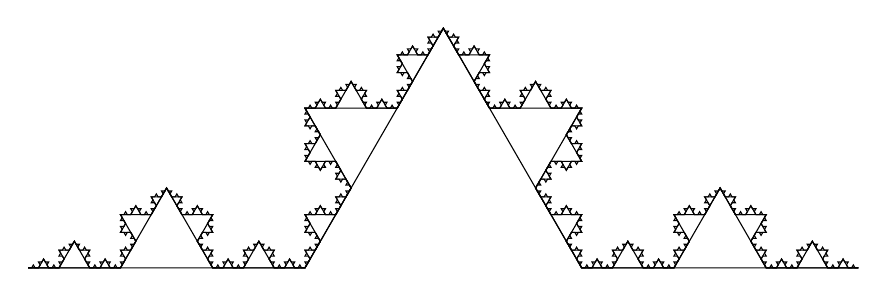
\begin{tikzpicture}
			\foreach \order in {1,...,5} {
					\draw<\order>[Koch curve={order=\order,step=300pt/3^(\order)}] l-system;
				}
		\end{tikzpicture}
	\end{center}
\end{frame}


\end{document}